\documentclass[11pt]{article}

\usepackage[portuguese]{babel}
\usepackage[a4paper,top=2cm,bottom=2cm,left=3cm,right=3cm,marginparwidth=1.75cm]{geometry}
\usepackage{amsmath}
\usepackage{graphicx}
\usepackage{float}
\usepackage[colorlinks=true, allcolors=blue]{hyperref}
\usepackage{listings}
\usepackage{hyphenat}
\usepackage{xcolor}

\title{\textbf{Projeto de Pesagem Automatizada de Gado (Sem título)}}
\author{
    Renan da Silva Oliveira Andrade (\texttt{renan.silva3@pucpr.edu.br})\\
    Ricardo Lucas Kucek (\texttt{ricardo.kucek@pucpr.edu.br})\\
    Pedro Senes Velloso Ribeiro (\texttt{pedro.senes@pucpr.edu.br})\\ 
    Riscala Miguel Fadel Neto (\texttt{riscala.neto@pucpr.edu.br})\\ Victor Valerio Fadel (\texttt{victor.fadel@pucpr.edu.br})
}

\begin{document}
\maketitle

\section{Descrição do contexto}

Em propriedades rurais, o controle de pesagem do corpo pecuário é indispensável para a manutenção da qualidade de vida dos animais. Controlar o peso dos bovinos/equinos ou quaisquer outros animais infere avaliar o desempenho em relação ao ganho de peso dos mesmos, algo de extrema importância para a pecuária comercial, pois impacta diretamente em sua produtividade e na lucratividade.

O controle de pesagem permite avaliar e ajustar a distribuição alimentar dos animais, garantindo que estes se desenvolvam de forma saudável. Em propriedades que trabalham com equinos, como haras e fazendas de criação, a pesagem auxilia na divisão correta da alimentação, suplementos e medicações, evitando sub ou sobrepeso, o que pode comprometer a saúde e a performance destes animais.

Além disso, o controle periódico do peso pode indicar animais que perderam peso de forma mais acentuada que o usual, fator este que pode alertar os criadores e cuidadores sobre possíveis doenças e evitar a piora do animal ou a possível disseminação da doença entre os demais animais, permitindo uma intervenção precoce e um manejo sanitário mais eficiente.

Em suma, o controle de pesagem dos animais nas propriedades rurais reflete-se diretamente no controle da qualidade da vida animal e na rentabilidade em propriedades rurais de cunho comercial.

\section{Problemática}
\section{Motivação}
\section{Proposta}
\section{Tecnologias envolvidas}
\section{Resultados esperados}
\section{Cronograma}

\begin{figure}[H]
    \centering
    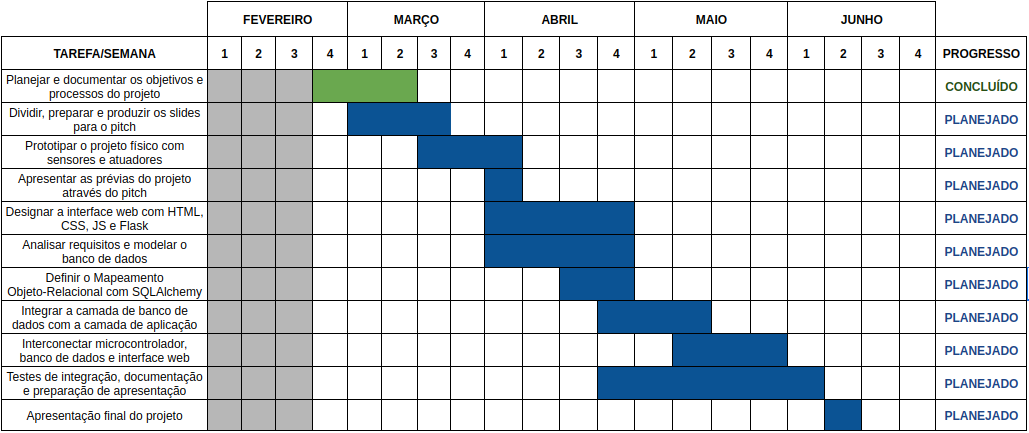
\includegraphics[width=0.9\linewidth]{cronograma.png}
    \caption{Cronograma}
\end{figure}

\bibliographystyle{apalike}
\bibliography{sample}

\end{document}
